\chapter{Analysis }

The following chapter will provide the business background of the project and further justification for such a system to be implemented, an analytic insight to the steps required for designing the proposed software in relation to a business use case, identify some of the problems that may arise and outline objectives for implementation.

\subsection*{Project Background}
An article by \citeauthor{hague} for the B2B international states that understanding a customer's satisfaction rate is important as it can show where is the business is doing well or where it needs improvements. It also can give indication to business owners where a further staff training is needed, or how there may be a need for cultural change. In light of this, seeing your business through the eyes of the customer can provide understanding of its downfalls. This in turn prevents more customer churn and can prove to be financially beneficial \citep{hague}. They state that the downfalls of customer service surveys is the that the survey must "ask the right question of the right person". \citeauthor{hague} give two reasons why this is difficult: they may not know what to ask the customer in respect to their specific interaction with the business, also they may not have the contact details of the customer to further inquire into satisfaction of the individual. A main reason why customer surveys result may be misleading is the fact that an average of only 10\% percent of online surveys sent to customers are responded to, meaning that these results are not representative of an entire customer base \citep{willott} . Furthermore, surveys are described by \citeauthor{hague} as a "snapshot at one point in time", and do not accurately represent the feelings of the customer during transaction process, and measuring the satisfaction of customers should "be a continuous process". \citeauthor{keith} (2017) describes the use of artificial intelligence technologies in customer service as a beneficial factor for businesses, as it can automate the tasks that are "too time consuming".

In consideration of the aforementioned problems in the customer service sector, the proposed technologies aim to eliminate the process of requesting customers to fill out surveys by performing a facial sentiment analysis during the transaction, and in turn reduce customer churn and the cost of marketing teams investing funds onto campaigns that me be driven by misleading or inaccurate data. In order to achieve the end goal of this project, a number of factors should be addressed. These consist of the type of model that should be implemented, what machine learning library should be used, which programming language is preferable for this project, how may the model be trained and what are the options for deployment. For these problems to be address, the project analysis shall be decomposed in to four components: The Machine Learning model, Data preparation, Training and Hosting/Deployment


%-collecting facts
%	- CNNs are used for CV
%	- They are trained on large data sets
%	- Models usually need a ML library
%	- A programming language is needed
%	- Can be hosted on server for production use
 	
%-identifying problems
% 	- How do i get a dataset?
% 	- What machine library should be used?
% 	- which programming language?
% 	- What PaaS should be used?
% 	- how can i train without high performing - GPU power?
 	
%-decomposition of problem into components 
%	- Neural Network model
%	- Data Preparation
%	- Training
%	- Hosting/Deployment

%-identifying objectives
%	- implement a CNN
%	- Acquire or create a dataset
%	- Train the model (locally or on cloud)
%	- Create python API for hosting trained model
%	- Create web app for user interaction

\section{The Machine Learning Model}


\subsection{Algorithm}
When dealing with image a classification problem such as facial sentiment analysis, there are two machine learning algorithms that deem worthy. Deep Belief Networks (DBN's) were developed as an alternative to back propagation by Geoff Hinton. The idea behind DBN's involves the stacking of a Restricted Boltzmann Machines in order to train in a "greedy manner" \citep{dbn}. This model learns to excerpt hierarchical representations of training data. The second algorithm is convolutional neural networks (CNN's). % As explained in the literature review, a CNN's consist of a number of convolution and sub-sampling layers. It is then followed by a dense, or otherwise known as, a fully-connected layer. It also uses back-propagation to adjust the weights of the network during training \citep{gupta}. 
To understand the structure of convolutional neural networks, firstly it should be briefly explained how an artificial neural network works.

\subsubsection{Artificial Neural Networks and Back Propagation}
Artificial Neural networks are based on the biological brain and possess a number of connected nodes. An artificial neural network can be seen as an hierarchical ordering of mathematical constructs called neurons, which are nodes that perform a mathematical function to simulated the biology of the brain on a molecular level \citep{muir}.  A neural network in one of it's most simplest of forms has 3 levels of structure, which are otherwise known as layers. The first layer consists of the neurons that takes in the data. This is called the input layer. This layer can consist of one or more nodes, depending on the number of inputs. The second component in the network is called the hidden layer. Unlike the input layer, hidden layers are considered as active as they can modify data as it passed through them \citep{smith_2011}. The input layer and the hidden layer are connected through what are known as weights. These weights are values that are randomly initialized. When passing data to the next layer of nodes, a set of matrix operations are done by multiplying the input data by the weight value. A bias is then added to the result of this. An activation function is then introduced to apply nonlinearity. Nonlinearities are used as they can provide methods of solving complex problems \citep{raschka_2016}. There are several activations that can be used such as Sigmoid, Tanh and Rectified Linear Unit (ReLU) to name a few. However, it has been noted that ReLU provides the best results as prevents issues such as the vanishing gradient problem. The activation of a neuron in a network can be described as the following \citep{collis_2017}:

\begin{equation}\label{eq:act}
output = activation function((input * weights) + bias)
\end{equation}

These steps are repeated for each neuron in the network until a predictive output is produced. This process, in full, is called forward propagation. From this output we can evaluate it to the true expected output to optimize the network. This is part of a process known as back propagation. Back propagation is expressed as the partial derivative of the cost/loss function, in respect to the any weight or bias that can be found within the network \citep{nielsen_2015}. In simplistic terms it can be defined as a function for adjusting the weights in the network to minimizing the loss functions values. This is done through what is known as the delta rule. The formula for adjusting these new weights are as follows:
\begin{equation}\label{eq:act}
New\ weight\ value = weight\ + learning\ rate\ x\ error\ x\ input\ value
\end{equation}

There are a wide range of optimization algorithms that can be used for this, the most popular of which is known as gradient descent \citep{walia_2017} where we calculate the gradient of the error with respect to the weights. When visualized, the gradient of the error will be equal to zero when the model finds the local minima and the network converges. An example of this can be seen in Figure \ref{grade}.

\begin{figure}[ht]
	\begin{center}
		\advance\leftskip-3cm
		\advance\rightskip-3cm
		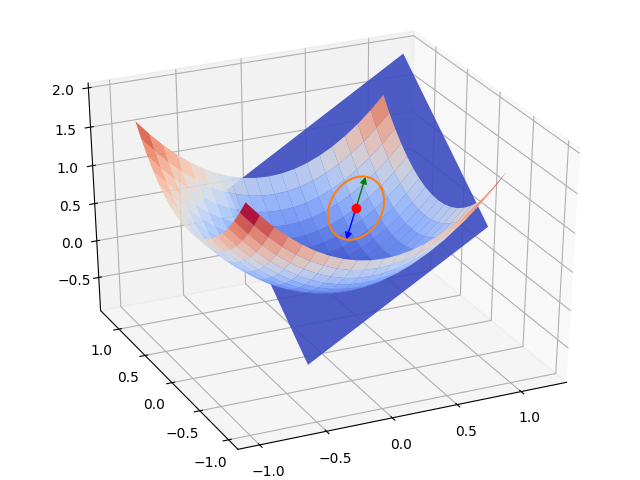
\includegraphics[keepaspectratio=true,scale=0.8]{__resources/design/gd.png}
		\caption{Gradient Descent Visualized by \cite{vigier_2017}}
		\label{grade}
	\end{center}
\end{figure}

\subsubsection{Convolutional Neural Networks}

A convolutional neural network (CNN) is a form of neural network used primarily for image classification and object recognition. CNN's, like regular artificial neural networks, take biological inspiration as they are based on visual cortex \citep{adit}. CNN's recognize images as three-dimensional objects (or two dimensional if the image is grayscaled). CNN's are made up of a number of components, which include the convolution layers, pooling layers and fully connected layers. Convolution layers are the first in the sequence of components. As explained by \citeauthor{adit}, the convolution layer should be thought of as a flash light being shined on a certain region of a picture from the top left to bottom right. This analogical flash is referred to as the feature filter or the kernel. This kernel convolves (slides) over the image and multiplies the images pixel values by the values in the filter, in a process which is known as element wise multiplication \citep{adit}. After this image is fully convolved, this results in what is known as a feature map. The second step is referred to as pooling, which is used for down sampling. This is necessary when dealing with highly spatial images age it reduces the data needed to be processed by the network \citep{kar}. The most popular approach for pooling is max-pooling, where the maximum pixel value found in the kernel (filter) is used as input for the next layer. The last component in the architecture is the fully connected layers. These layers take the output from the layer convolution or activation layer preceding it. Each node in the network is connected to every other node following it, hence the name "fully connected". From here the network act the same way as a regular multilayer perceptron ANN.




\subsection{Programming Language}
There are many programming languages that can used for machine learning and artificial intelligence. \citeauthor{brownlee} (2016) describes the quest for choosing a programming language to be rather difficult, as the choice should be tailored around "your own requirements" and entirely depends on the project being undertaken. However, opinions on popular machine learning languages are given. Firstly, MATLAB/Octave is described as being "excellent" for dealing with matrices and linear algebra \citep{brownlee}. The R language is shown to be a prominent choice for machine learning as it provides many machine learning algorithms and it is a great choice for developing advanced models. \citeauthor{brownlee} (2016) states, although it is a good choice, it is seen as having a hard learning curve at first use. Python is said to be competition to MATLAB and R as it's large range of libraries and abilities as widely used in the field of data science \citep{brownlee}.
An article by \citeauthor{verma_2017} (2017) sheds light on most popular programming languages in terms job listings for the year of 2016. Coming in first place was Python, as it's popularity is unmatched by any other programming language. Following Python is Java, then R is seen to be the third most popular \citep{verma_2017}. See Figure \ref{verma} for graphical representation \citeauthor{verma_2017}'s findings.

\begin{figure}[ht]
	\begin{center}
		\advance\leftskip-3cm
		\advance\rightskip-3cm
		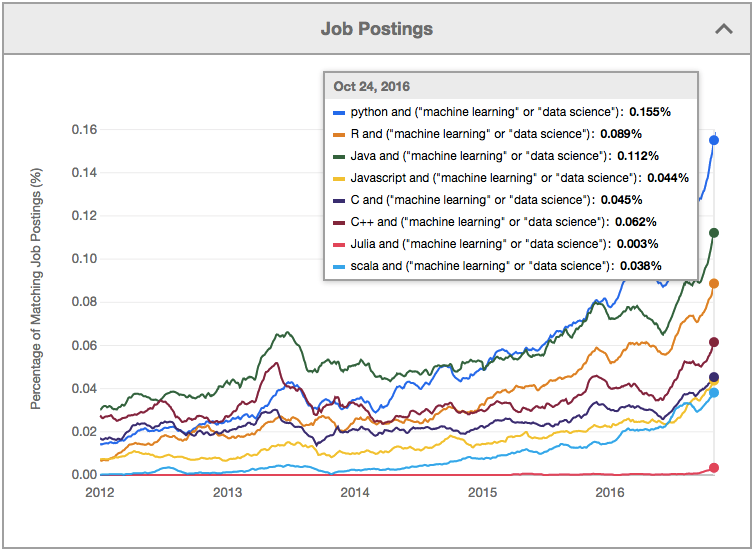
\includegraphics[keepaspectratio=true,scale=0.6]{__resources/research/top_lang.jpg}
		\caption{Graph of Machine Learning or Data Science Languages for 2016 by \cite{verma_2017}}
		\label{verma}
	\end{center}
\end{figure}

In light of the proclamations made above, it is clear that the preferred languages should be easy to learn, are backed by a large community, and is capable of complex mathematical operations. Also, it is desirable that the languages chosen for the proposed language is fast and efficient because of the complex computations that will occur during training.

\newpage

\subsection{Machine Learning Library}
To speed up the process of implementation, a machine learning (ML) should be used. This will speed up the process of the project as many ML libraries have API's to help eliminate tedious tasks. Also, these can be used to reduce the complexity and the length of the program \citep{jain}.
TensorFlow is an open source ML library developed by the Google Brain team. It can be run on CPUs, GPUs and mobile platforms. For machine learning algorithms, such as gradient descent, TensorFlow provides automatic differentiation which can prove to be very advantageous in comparison to other ML libraries. It also supports multiple languages such as Python, Java and C++ and Go \citep{jain}. Graph visualisation is also supported. Multi-threading is also achievable with the use of TensorFlow \citep{jain}. Higher level wrapper libraries such as Keras can use back-end API's such as TensorFlow provide easier implementation with minimalistic coding but also giving the same efficiency and accuracy \citep{lee_keras}. Scikit Learn is an open source ML library built on top of other libraries such as Matplotlib, SciPy and NumPy. A good feature that Scikit Learn incorporates is the ability of evaluating, chaining and adjusting model hyper parameters \citep{jain}.
Other ML libraries such as Caffe focuses on speed and modularity and is mainly utilized for convolutional neural networks and computer-vision. Another selling point for Caffe is it's pre-trained models that do not require any coding or training and it supports GPU and CPU computations. A disadvantage of this library is that it is specifically designed for application implementation, not for research and development \citep{jain}.

\section{Dataset}
For this project, the machine learning model will require a large image dataset. This dataset will be used to train the model on certain facial feature expressions with supervised learning, therefore a labeled dataset is needed. Acquiring a good dataset is one of the most important parts of the project, as the model only as good as the data you train it with \citep{capg}.

\subsection{Public Datasets}
As seen in the literature review, there are very few datasets publicly available for use on the Internet that provide labeled data. For example, the CK+ dataset was used by \citeauthor{LOPES} used labeled data to train their model. The dataset included facial expressions such as sadness, surprise, happiness, anger, fear and disgust. Which is a considerable approach for training the model.

\subsection{Creating a Dataset}
Creating a dataset is another option for training the model. A number of images could be batch downloaded from image search engines such as Bing or Google and split into training and testing sets. As for labeling, the name of the folder the type of picture is in will serve as the label.

\section{Training}
Training is a vital part of the project and will be the most time consuming. The model will use the chosen data preparation method and use that data as input to the model. There are two ways the model can be trained: Locally and on an Infrastructure as a Service (IaaS).

\subsection{Training Locally}
Training locally involves running code on your own machine to train the model. A main advantage to this is that it is low cost. There are no fees in this approach besides the electricity used by the machine. However, this approach may be harmful to the machine as the high rate of computations produces a lot of heat, which may prove to be detrimental to your hardware. Also, should the machine not have the sufficient hardware, such as a high-performing graphical processing unit (GPU), the training elapse time will be significantly larger.

\subsection{Cloud Training}
Training in the cloud involves uploading the model code and dataset to a cloud platform service. These infrastructures provide dedicated hardware for machine learning training such as high-performance GPU's and CPU's. They usually provide container environments to run the training. For example, should a model be implemented in Keras or Caffe, the platforms have dedicated runtime environments with these libraries pre-installed. Notable platforms for machine learning training are TensorPort, FloydHub and Amazon's AWS. Although it is faster to train a model on one of these platforms, they can be expensive, as the free tiers only provide a certain amount of free server usage time.

\section{Hosting/Deployment}
Deployment of the trained model is required to serve it as a web service endpoint. This model should be hosted as an API to enable use from devices besides the machine it was trained on. The API will require a platform that containerizes and supports the machine learning libraries it was used to train with. Additionally, the API should be lightweight and fast for accurate classifications. There are many Platforms as a Service (PaaS) that can be used for this project, notably Heroku, AWS, Azure and Google App Engine all provide a free tier basis for deployment.


\section{Concluding Objective}
In conclusion, this section outlines the objectives for the proposed project sequentially from the initial steps to the end product. The objectives are as follows:

\begin{itemize}
	\item Acquire a suitable dataset of facial expression images.
	\item Build a convolutional neural network for facial expression classification using an ML library.
	\item Train the model on a large image data set.
	\item Save the trained model and deploy it as an API.
	\item Develop a web application that is enabled to record a user's facials expressions
	\item Use image pre-processing on the web cam images for more accurate predictions.
	\item Send snapshots of the users face to the Python API in intervals, classify them and display the results to the user.
	%\item Use tone analyzer API for voice sentiment recognition.
	%\item Weigh scores from the train model and tone analyzer accordingly and store them in a database
\end{itemize}

